Riprenderei appunti di Russo e basta. Riportiamo cmq quello che dice lei.
Ci sono quattro principi base nella relatività.
\begin{itemize}
    \item Ogni legge fisica è invariante in ogni sistema di riferimento inerziale.
    \item Energia, impulso, momento angolare in ogni sistema fisica isolato si conservano.
    \item La velocità della luce è la stessa in ogni sistema di riferimento.
    \item Il tempo non è invariante (assoluto).
    \item I primi due sono legati alla meccanica classica, gli ultimi due alla relatività. Da ciò ne segue che le trasformazioni galileiane non valgono più, e al loro posto ci sono le trasformazioni di Lorentz. Nel limite $\beta\ll1$ le trasformazioni di Lorentz diventano quelle di Galileo.
\end{itemize}
\subsection{Trasformazioni di Lorentz}
\begin{itemize}
    \item Definiamo i quadrivettori come $A=(a_0,a_i)=(a_0,\vec a)$, con $a_0$ componente temporale e $a_i$ componente spaziale.
    \item Definiamo il prodotto scalare tra quadrivettori come $\tilde A\tilde B =a_0b_0-a_ib_i$. Questo prodotto è invariante sotto trasformazioni di Lorentz.
    \item Se consideriamo un sistema di riferimento $S$ e un altro $S'$, con $S'$ che si muove rispetto a $S$ con velocità $v$ lungo l'asse $x$, allora le trasformazioni di Lorentz sono date da:
    \begin{equation*}
        \mqty(a'_0 \\\xmat*{a'}{3}{1})= 
        \underbrace{\begin{pmatrix}
            \mqty{\gamma & -\beta\gamma & 0 & 0 \\ -\beta\gamma & \gamma &0&0 \\ 
            0 & 0 & 1 & 0 \\ 
            0 & 0 & 0 & 1 }
        \end{pmatrix}}_{=L(\beta)}
        \mqty(a_0 \\\xmat*{a}{3}{1})= 
        \mqty(\gamma a_0-\beta\gamma a_1\\-\beta\gamma a_0+\gamma a_1\\a_2\\a_3)\implies 
        \begin{cases}
            ct'=\gamma(ct-\beta x) \\
            x'=\gamma(x-\beta ct)
        \end{cases}
    \end{equation*}
    Una proprietà importante è $L(\beta)^{-1}=L(-\beta)$, da cui ne segue che per invertire le trasformazioni di Lorentz basta scambiare variabile con indice con quelle senza e $\beta\to-\beta$.
    \item Che si ha al limite non relativistico? Supponiamo $\beta\ll1\implies\gamma\approx1+\frac{\beta^2}{2}\approx1$. Ne segue per il tempo che
    \begin{equation*}
        ct'=\qty(1+\frac{\beta^2}2)(ct-\beta x) \approx ct-\beta x + \frac{\beta^2}2ct\approx ct\implies t'=t 
    \end{equation*}
    e per lo spazio che 
    \begin{equation*}
        x'=\qty(1+\frac{\beta^2}2)(x-\beta ct)\approx x-\beta ct\implies x'= x - vt
    \end{equation*}
    \item Se il moto non è solo lungo $x$, allora dobbiamo considerare $\vec\beta=\frac{\vec v} c$ e 
    \begin{equation*}
        \begin{cases}
            ct'=\gamma(ct-\beta x_\parallel) \\
            x'_\parallel=\gamma(x_\parallel-\beta ct)\\
            \vec x_\perp'=\vec x_\perp
        \end{cases}
    \end{equation*}
    \item Dimostriamo che il prodotto scalare è invariante. Sia $A=(a_0,\vec a)$ e $B=(b_0,\vec b)$. Calcoliamo $A'\cdot B'$.
    \begin{equation*}
        A'\cdot B'=a_0'b_0'-\vec a'\cdot\vec b'=\gamma^2(a_0-\beta a_1)(b_0-\beta b_1)-\gamma^2(a_1-\beta a_0)(b_1-\beta b_0)-a_2b_2-a_3b_3=\dots=A\cdot B
    \end{equation*}
\end{itemize}
Vediamo alcune conseguenze in high energy physics.
\begin{itemize}
    \item La contrazione delle lunghezze. Consideriamo un oggetto di lunghezza $L$ che si muove con velocità $v$. Supponiamo che il sistema solidale ad esso sia $S'$ e la lunghezza misurata sia $d'=x_2'-x_1'$ che avviene simultaneamente quindi $t_2=t_1$. Se trasformiamo otteniamo $d'=x_2'-x_1'=\gamma(x_2-\beta ct_2)-\gamma(x_1-bct_1)=\gamma(x_2-x_1)-\gamma\beta c(t_2-t_1)=\gamma(x_2-x_1)=d\implies d'=\gamma d$. Ne segue che la lunghezza misurata da un osservatore in moto è contratta di un fattore $\gamma$, e la lunghezza propria, misurata nel sistema solidale all'oggetto è la massima possibile.
    \item La dilatazione temporale. Consideriamo due eventi che avvengono nello stesso punto nello spazio, ma in tempi diversi. Se trasformiamo otteniamo $c\Delta t=c(t_2-t_1)=\gamma c(t_2'-t_1')+\beta \gamma (x_2'-x_1')=\gamma c\Delta t'$. Ne segue che il tempo misurato da un osservatore in moto è dilatato di un fattore $\gamma$, e il tempo proprio, misurato nel sistema solidale all'oggetto è il minimo possibile. Da ciò si hanno varie conseguenze.
\end{itemize}
\subsection{Esperimento CPP, muoni, pioni e Yukawa}
\begin{itemize}
    \item Nel 1912 Hess scoprì i raggi cosmici. Nel 1932 Anderson scoprì i positroni, predetti da Dirac nel 1928 (già discussa).
    \item Nel 1935 Yukawa introdusse la teoria delle interazioni forti, predicendo una massa mediatrice di $\sim 100$ MeV. Il mesone di Yukawa doveva decadere in elettrone e netruino con tempo di decadimento di $\sim1\mu$s. Nel 1937 si scoprì il mesotrone (Anderson e Neddermeyer), con una massa di $110$ MeV, associata alla particella di Yukawa. Nel 1940 si studiò assorbimento e decadimento delle proprietà di assorbimento del mesone di Yukawa.
    \item Il decadimento del mestrone (che in realtà è un $\mu$) fu studiato diverse volte. Nel 1940 si osservò il suo decadimento in positroni; nel 1941 ci fu una misura da Rasetti che ottenne $\tau=(1.5\pm0.3)\mu$s. Nel 1941 Piccioni e Conversi decisero di lavorare assieme e migliorare la precisione nella misura del tempo di decadimento (del mesone di Yukawa).
    \item Nel 1939 Montgomery fece un esperimento (\autoref{fig:montgomery}) per misurare il decadimento del $\mu$
    \begin{figure}[h]
        \centering
        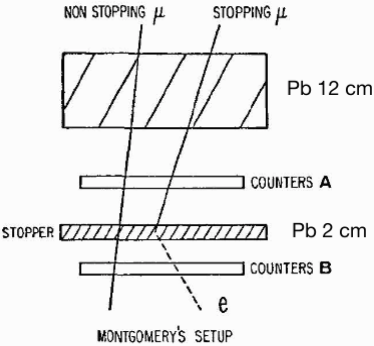
\includegraphics[width=0.4\textwidth]{immagini/fig_montgomery.png}
        \caption{Esperimento di Montgomery. Volevano estrarre il tempo di decadimento dalle intensità delle coincidenze ritardate con e senza stopper. Purtroppo non riuscirono a misurare il tempo di decadimento del $\mu$ a causa del troppo rumore in B.}
        \label{fig:montgomery}
    \end{figure}
    \item Un altro tentativo fu fatto da Rasetti nel 1940, con un apparato più complicato (\autoref{fig:rasetti}).
    \begin{figure}[h]
        \centering
        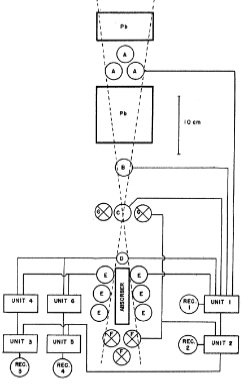
\includegraphics[width=0.4\textwidth]{immagini/fig_rasetti.png}
        \caption{Disposizione dei contatori, illustrando le connessioni con gli amplificatori.}
        \label{fig:rasetti}
      \end{figure}
    Nella procedura sperimentale si definisce un fascio di mestroni con la coincidenza ABCD. L'anticontatore G discrimina dagli sciami elettromagnetici. L'anticontatore F seleziona i mestroni che si sono fermati nell'assorbitore. Il contatore E rivela particelle emesse nell'assorbitore. Non si usarono coincidenze ritardate ma "immediate" con tempi di risoluzione diversi. Guardando le combinazioni dei tempi con cui il segnale arriva, hanno fatto un fit particolare ed estratto il tempo di decadimento. Ottennero $\tau=(1.5\pm0.3)\mu$s.
    \item Successivamente l'esperimento fu riproposto da Conversi, Pancini e Piccioni con l'idea di effettuare una misura migliore (vedi \autoref{fig:cpp})
    \begin{figure}[h]
        \centering
        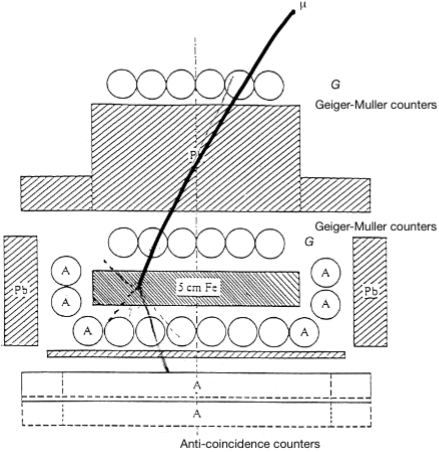
\includegraphics[width=0.4\textwidth]{immagini/fig_cpp.png}
        \caption{}
        \label{fig:cpp}
      \end{figure}
    Un mesotrone si ferma nell'assorbitore (Fe) e poi decade. Si usano coincidenze ritardate tra i contatori sopra e sotto e le anticoincidenze (A). Gli elettroni si fermano nell'assorbitore di Pb. Le anticoincidenze servono a scartare l'evento. Misurarono $\tau=(2.33\pm0.15)\mu$s, meglio di Rasetti. 
\end{itemize}
    Torniamo ai quadrivettori. 
    \begin{itemize}
    \item La matrice della metrica la conosciamo è $g^{\mu\nu}=\text{diag}(1,-1,-1,-1)$. Un quadrivettore importante è quello di impulso $P^\mu=(E,\vec p)$. Questo quadrivettore non è invariante ma il suo quadrato sì. Facendolo, scopriamo che vale $P^\mu P_\mu=m^2$ usando la relazione di mass-shell.
    \item Alcune relazioni utili sono: $p=\gamma mv$, $E=\gamma m$, $T=mc^2(\gamma-1)$, $\beta=\frac p E$.
    \item Quando facciamo esperimento di fisica di particelle, ci mettiamo nel riferimento di laboratorio solidale all'osservatore e ai rivelatori. In questo riferimento tipicamente $v\_T=0$. Possiamo scrivere allora nel riferimento del laboratorio $P_1=(E_1,\vec {p}_1)$, $P_2 = (m\_T,0)$ (1 = proiettile, 2 = target). Allora $P\_{tot}=sP_1+P_2=(E_1+m\_T,\vec p_1)$. 
    \item Un altro sistema di riferimento utile è quello del centro di massa, in cui $\vec {p}\_{tot}=0$. Se consideriamo una particella incidente in un target, avremo $P_1^*=(E_1^*,\vec p)$ e $P_2^*=(E_2^*,-\vec p)$. Allora $P\_{tot}^*=(E_1^*+E_2^*,0)$. Poichè è un invariante, $P\_{tot}^2$ sarà uguale nel riferimento del centro di massa e in quell del laboratorio. Ne segue che $P\_{tot}^{*,2}=E^2\_{CM}=P\_{tot}^{\text{lab},2}=(E_1+m\_T)^2-p_1^2=E_1^2+m\_T^2+2E_1m\_T-p_1^2=m_1^2+2E_1m\_T+m\_T^2$. ('sta roba è inutile?)
    \item Se consideriamo un fascio di $n$ particelle allora dovremo considerare la sommatoria. $P_\mu P^\mu= (E_1+E_2+\dots+E_n)^2-(\vec p_1+\vec p_2+\dots+\vec p_n)^2$ in generale. Se consideriamo il sistema del centro di massa avremo $P^{\mu,*}=(E\_{CM},0)$. Quindi nel riferimento del centro di massa questo scalare è solo il quadrato dell'energia nel sistema del centro di massa.
    \item Riprendiamo la storia. Nel 1947 ci fu la scoperta del pione, usando le emulsioni nucleari. Decade in sequenza il pione in muone ed infine in elettrone. In tutti gli eventi il muone aveva energia di 4.1 MeV a cui corrisponde il range misurato di 600 $\mu$m, le strisce sono tutte di uguale lunghezza (sappiamo da Bethe-Bloch che il range e l'impulso sono legati). In base a densità di ionizzazione ($\dd{E}/\dd{x}$) distinguiamo il tipo di particella.
    \item Visto che il range è sempre lo stesso, l'impulso del muone sarà sempre lo stesso 29 MeV. Visto che l'impulso è sempre lo stesso, il decadimento deve essere a due corpi (e non tre altrimenti si avrebbe spettro continuo). 
    \item Supponendo che si abbia un decadimento a due corpi con la particella iniziale che si ferma, abbiamo $X\to\mu+\nu_\mu$ e il sistema del centro di massa coincide con il sistema solidale a $X$ (il $\pi$). Da ciò ne segue che impulso di neutrino e muone sono uguali ed opposti, quindi  
    \begin{equation*}
    m\_X^2=E\_{cm}^2=(E_\mu+E_\nu)^2\implies m\_X=\sqrt{m_\mu^2+p_\mu^2}+p_\nu=\dots=138.9 \text{ MeV}
    \end{equation*}
    \item Il decadimento $\pi^-\to\mu^-+\bar\nu_\mu$ è dovuto alla forza debole, lo si capisce dal fatto che da quando avevo quark e antiquark, nei prodotti non li avrò più cioè non conservano il flavour. Un altro modo per capirlo è dai tempi di decadimento. 
    \begin{enumerate}
        \item Debole $10^{-8}-10^{-10}$ s.
        \item Elettromagnetico (come $\pi^0\to \gamma+\gamma$) $10^{-17}-10^{-16}$ s.
        \item Forti $10^{-22}-10^{-23}$ s.
    \end{enumerate}
\end{itemize}
Parliamo di processi virtuali e reali. 
\begin{itemize}
    \item Supponiamo di avere $e^-\to\gamma+e^-$. Abbiamo inizialmente (nel riferimento solidale all'elettrone) $e^-(m_ec^2,\vec0)$, invece dopo l'interazione abbiamo $e^-(E_k,-\vec k)+\gamma(c\abs{\vec k},\vec k)$. Valutiamo $\Delta E= ck+\sqrt{(m_ec^2)^2+(ck)^2}-m_ec^2$ consderando i due casi limite:
    \begin{enumerate}
        \item $ck\ll m_ec^2\implies \Delta E \gtrapprox ck$
        \item $ck\gg m_ec^2\implies \Delta E \lessapprox 2ck$
    \end{enumerate}
    Ne segue che 
    \begin{equation*}
        kc\leq\Delta E\leq2kc
    \end{equation*}
    ma ciò che importa è che $\Delta E\neq0$. Questo è un processo virtuale che non può avvenire da isolato. È possibile per un tempo compatibile con il principio di indeterminazione $t<\frac\hbar{\Delta E}$, a cui corrisponde uno spazio percorso $l=ct=\frac{c\hbar}{\Delta E}\propto(\Delta E)^{-1}$.
    \item Consideriamo un generico processo di scambio $A+B\to A+B$ che avviene tramite $X$. Avremo inizialmente $A(m_Ac^2,\vec0)$, invece dopo $A(E_p,\vec p)+X(E_X,-\vec p)$ e uguale per B. Vediamo quanto vale $\Delta E= E_X+E_p-m_Ac^2$ e i due casi limite:
    \begin{enumerate}
        \item $p\to\infty\implies \Delta E=2pc$
        \item $p\to0\implies\Delta E \geq m_Xc^2$
    \end{enumerate}
    ne segue che vale sempre $\Delta E\geq m_Xc^2$. Abbiamo detto che si può violare la conservazione dell'energia per $t\sim\frac\hbar{\Delta E}\implies l=\frac{c\hbar}{\Delta E}\approx\frac\hbar{m_X}$, dove $l$ è la massima distanza raggiungibile dal mediatore $X$ prima di essere ri-assorbito, e corrisponde esattamente al \textit{range della interazione}. 
    \item Viceversa, se conosco il range della interazione posso trovare la massa del mediatore! La relazione dunque è $R=\frac\hbar{m_Xc}$. Cerchiamo la massa del mediatore della interazione forte, supponendo che abbia $R\approx 1.2$ fm. Abbiamo 
    \begin{equation*}
    m_X=\frac1R=140\text{ MeV}
    \end{equation*}
    che è il mesotrone di Yukawa, chiamato così perché aveva massa intermedia tra $p$ ed $e^-$ (uniche particelle note oltre a $n$).
    \item Dunque se la massa del mediatore è nulla, il range dell'interazione è infinito (interazione elettromagnetica con fotoni). Se invece usiamo la massa del $W$, troviamo il range dell'interazione debole 
    \begin{equation*}
    R\_{debole}=\frac{\hbar c}{m_Wc^2}=\frac1{m_W}=\frac{200\text{ MeV}\cdot\text{fm}}{80\cdot 10^3\text{ MeV}}=2.5\cdot10^{-3}\text{ fm}
    \end{equation*}
    ben tre ordini di grandezza inferiori rispetto a quello nucleare.
    \item In passato si aveva una visione errata del $\beta$-decay, ad esempio $n\to p+e^-+\bar\nu$. In realtà questo avviene con uno scambio di $W^-$, cioè il neutrone (in realtà è tra quark) emette un $W^-$ diventando un $p$, e contemporaneamente $W^-\to e^-+\bar\nu$. Tuttavia questo processo lo trascuriamo a basse energie (MeV) in quanto irrilevante. 
\end{itemize}
Torniamo alla parte storica e all'esperimento CPP.
\begin{itemize}
    \item Abbiamo detto che l'esperimento CPP è importante perché da una migliore misura di $\tau_\mu$, ma c'è un altro motivo per cui è importante.
    \item Nel 1940 Tomonaga e Araki proposero una teoria, che fu accettata da tutti, sull'interazione forte. Il mesone di Yukawa interagisce con il nucleo mediante interazione forte. Secondo i calcoli, la cattura nucleare dipende leggermente dallo Z del materiale. I mesotroni positivi sono respinti dal nucleo, mentre quelli negativi possono essere catturati, ne segue che i mesotroni positivi possono soltanto decadere.
    \item  Per testare questa teoria che prevedeva una asimmetria tra mesotroni positivi e negativi, si usò lo stesso apparato CPP. La differenza stava in assorbitori più sottili (0.6 cm di Fe invece di 5 cm) per migliorare la efficienza di rivelazione degli elettroni. Misurarono il rapporto di mesotroni che decadono dentro il ferro che era in accordo con il valore aspettato (da raggi cosmici si aspettavano un eccesso del 20\%).
    \item Poi ripetettero l'esperimento con un apparato migliore utilizzando le lenti magnetiche per separare mesotroni positivi e negativi. Con un assorbitore ad alto Z (ferro) ci fu conferma della teoria, con uno a basso Z (carbonio), per completezza e per rivelare i fotoni emessi da cattura nucleare dei mesotroni negativi, invece ci fu disaccordo. Quindi la differenza è il campo magnetico che distingue i mesotroni positivi e negativi e utilizzo di assorbitori con alto e basso Z.
    \item Attraverso assorbitori di 5 cm di Fe c'è accordo perché la frequenza di decadimento è maggiore per quelli positivi non catturati rispetto a quelli negativi, il cui risultato sperimentale è compatibile con zero (vengono catturati dai nuclei prima di decadere). Il problema nasce con assorbitori di grafite, perché si trova che il rate di decadimento delle particelle negative non solo è diverso da zero, ma molto simile a quelle positive. Allora i mesotroni non sono le particelle di Yukawa, quelle che interagiscono fortemente.
    \item Fermi e altri discussero, e conclusero che ci sono circa 12 ordini di grandezza di differenza tra il tempo di cattura per una particella di Yukawa negativa e i risultati dell'esperimento. Quindi il mesotrone fu ribattezzato, come lo conosciamo oggi, mesone $\mu$, ed oggi sappiamo che il pione è la particella di Yukawa.
    \item Quindi CPP è rivoluzionario perché scopre che il muone non è la particella di Yukawa, quindi è un altro leptone! Apre la strada alla seconda generazione di particelle, con cui si va oltre la materia ordinaria. Quindi è l'inizio della \textit{fisica delle particelle}.
\end{itemize}
Vediamo il potenziale di \textit{Yukawa}.
\begin{itemize}
    \item Consideriamo $A+B\to A+B$ con particella mediatrice $X$. Questa particella è un bosone, se in più la consideriamo relativistica allora obbedisce all'equazione di Klein-Gordon. Nel caso statico (stazionario) si riduce a
    \begin{equation*}
        \nabla^2\phi(\vec x)=\frac{m_X^2c^2}{\hbar^2}\phi(\vec x)
    \end{equation*}
    se la massa è nulla ritroviamo l'equazione di Laplace e quindi il mediatore è il fotone e la soluzione è il campo elettrostatico $V(r)=-\frac{e^2}{4\pi\varepsilon_0}\frac1r$. Se invece la massa non è nulla otteniamo $V(r)=-\frac{g^2}{4\pi}\frac{e^{-r/R}}{r}$ che è il \textit{potenziale di Yukawa} con il range $R=\frac{\hbar}{m_Xc}$. La forma del potenziale è simile a quello che si ottiene quando consideriamo effetti di schermaggio e vogliamo la carica effettiva subita dal sistema.
    \item Ci sono delle ipotesi su cui si basa il modello di Yukawa.
    \begin{enumerate}
        \item I nucleoni sono le sorgenti del campo nucleare e l'interazione tra essi avviene tramite scambio di bosoni che quantizzano il campo nucleare (detti mesoni).
        \item L'interazione è a corto range, con range legato alla massa della particella mediatrice.
        \item L'interazione nucleare è indipendente dalla carica elettrica.
        \item Il potenziale è a simmetria sferica e dipende anche dagli spin dei nucleoni (che abbiamo ignorato).
    \end{enumerate}
\end{itemize}
Il modello di Yukawa serve anche a spiegare lo scattering $p-n$.
\begin{itemize}
    \item La distribuzione angolare di scattering protone-neutrone ha un andamento a parabola con picchi in 0 e 180 gradi (e minimo in mezzo da qualche parte). Senza il modello di Yukawa non è spiegabile.
    \item Se lo scattering è elastico $\abs{\vec p_i}=\abs{\vec p_f}$. L'impulso trasferito varrà $\Delta p = \abs{\vec p_i-\vec p_f}=F\_{media}\Delta t$. Considerando il potenziale nucleare come una buca, avremo $F\_{media}=\frac{V_0}R$. La variazione di impulso è legata all'angolo soltanto visto che è elastico, quindi  (usando $\Delta t=R/v$)
    \begin{equation*}
        \Delta \vartheta\approx \frac{\Delta p} p=\frac{F\_m\Delta t}p=\frac{V_0}{vp}\implies \vartheta=\frac{V_0}{2E\_{cin}}
    \end{equation*}
    usando il valore tipico di $V_0=35$ MeV e $100$ MeV $\leq E\_{cin}\leq600$ MeV (usati sperimentalmente) otteniamo $\vartheta=10$ gradi, che è in accordo con i dati sperimentali. 
    \item Quindi con la cinematica spieghiamo il picco ad angoli bassi, ma non quello ad angoli alti. Per spiegarlo dobbiamo considerare il modello di Yukawa, si scambiano un pione quindi esiste uno stato intermedio (non è puntuale, pensando a diagramma di Feynman senza mediatore).
\end{itemize}